\documentclass{article}
\usepackage{amsmath}
\usepackage{xcolor}
\usepackage{ragged2e}
\usepackage{graphicx}
\usepackage{gensymb}
\usepackage{mathtools}
\newcommand{\mydet}[1]{\ensuremath{\begin{vmatrix}#1\end{vmatrix}}}
\providecommand{\brak}[1]{\ensuremath{\left(#1\right)}}
\providecommand{\norm}[1]{\left\lVert#1\right\rVert}
\newcommand{\solution}{\noindent \textbf{Solution: }}
\newcommand{\myvec}[1]{\ensuremath{\begin{pmatrix}#1\end{pmatrix}}}
\let\vec\mathbf
\begin{document}
\begin{center}
	\textbf\large{CHAPTER-7 \\ TRIANGLES}
\end{center}
\section{Exercise 7.1}
Q1. If $AB = QR$, $BC = PR$ and $CA = PQ$, then 
\begin{enumerate}
	\item  $\triangle{ABC} \cong \triangle{PQR}$
	\item  $\triangle{CBA} \cong \triangle{PRQ}$
	\item  $\triangle{BAC} \cong \triangle{RPQ}$
	\item  $\triangle{PQR} \cong \triangle{BCA}$
\end{enumerate}
\solution
According to the question,
\begin{align}
	AB = QR\\
	BC = PR\\
	CA =PQ
\end{align}
Since,
\begin{align}
	AB = QR\\
	BC = PR\\
	CA = PQ
\end{align}
This follows SSS criteria and we can say that, $A$ corresponds to $Q$, $B$ corresponds to $R$, $C$ corresponds to $P$ as shown in Figure:\ref{fig:Fig}.\\ \\
Hence, option 2 is the correct answer.
\begin{figure}[h]
	\begin{center}
		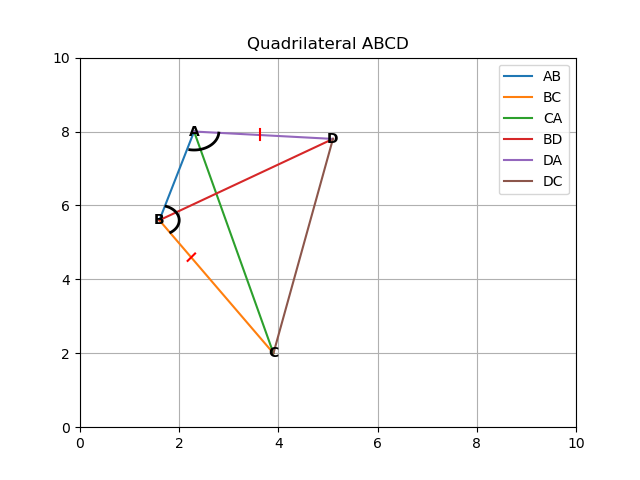
\includegraphics[width=\columnwidth]{figs/graph.png}
	\end{center}
	\caption{}
	\label{fig:Fig}
\end{figure}
\end{document}
